\documentclass[10pt]{article}

\usepackage[version=3]{mhchem} % Package for chemical equation typesetting
\usepackage{siunitx} % Provides the \SI{}{} and \si{} command for typesetting SI units
\usepackage{graphicx} % Required for the inclusion of images
\usepackage{natbib} % Required to change bibliography style to APA
\usepackage{nth}
\usepackage{amsmath} % Required for some math elements
\usepackage{tabulary}
\usepackage{graphicx}
\usepackage{floatrow}
\usepackage{chemfig}
\usepackage{float}
\usepackage[font={small}]{caption}
\usepackage[margin=1in]{geometry}
\setlength\parindent{0pt} % Removes all indentation from paragraphs

\renewcommand{\labelenumi}{\alph{enumi}.} % Make numbering in the enumerate environment by letter rather than number (e.g. section 6)

%\usepackage{times} % Uncomment to use the Times New Roman font


\title{Spectroscopy \\ \& Solutions \\ CHEM 1211L} % Title

\author{Chris \textsc{West}} % Author name

\date{\today} % Date for the report

\begin{document}

\maketitle % Insert the title, author and date

\begin{center}
\begin{tabular}{l r}
Date Performed: & June 14, 2017 \\% Date the experiment was performed
Partner: & Chris Tillis \\ % Partner names
Instructor: & Dr. MacGowan % Instructor/supervisor
\end{tabular}
\end{center}
\floatsetup[table]{capposition=top}

%----------------------------------------------------------------------------------------
%	SECTION 1
%----------------------------------------------------------------------------------------

\section{Experimental Data}
\begin{table}[H]
\resizebox{50em}{!}{
\begin{tabular}{|l|l|l|}
\hline
\multicolumn{1}{|c|}{{\ul{\textbf{Mass of plant matter (grams)}}}} &
\multicolumn{1}{c|}{{\ul{\textbf{Volume of distilled water (mL) used to extract dye from plant}}}} &
\multicolumn{1}{c|}{{\ul{\textbf{Concentration (g/mL) of plant extract}}}} \\
\hline
	20.05 g & 100 mL & .2 $\frac{g}{mL}$ \\ \hline
	\end{tabular}
	}
	\centering
\caption{Preparation of stock solution from cooked cabbage leaves}
\label{Table 1}
\end{table}
\hspace{5ex}Sample calculation for concentration of orange extract:
\begin{center}
Concentration = $\frac{(20.05 ml)}{100}$ = .2 $\frac{g}{mL}$ \\
Concentration = .2 $\frac{g}{mL}$\\
\end{center}
\begin{table}[H]
\resizebox{50em}{!}{
\begin{tabular}{|l|l|l|l|}
\hline
\multicolumn{1}{|c|}{{\ul{\textbf{Dilution factor for plant extract}}}} &
\multicolumn{1}{c|}{{\ul{\textbf{Concentration of plant extract (g/mL)}}}} &
\multicolumn{1}{c|}{{\ul{\textbf{Absorbance value}}}} &
\multicolumn{1}{c|}{{\ul{\textbf{$\lambda$ max (nm) of Absorbance value}}}} \\
\hline
	No dilution & .2 $\frac{g}{mL}$ & 2.187 & 431.3 nm \\ \hline
	Dilution 1:1 - 2 mL extract to 2 mL distilled \ce{H2O} & .1 $\frac{g}{mL}$ & 1.681 & 400.9 nm \\ \hline
	Dilution 1:2 - 4 mL extract to 8 mL distilled \ce{H2O} & .05 $\frac{g}{mL}$ & 1.268 & 400.0 nm \\ \hline
	\end{tabular}
	}
	\centering
\caption{Absorbance data for various dilutions of plant extract}
\label{Table 2}
\end{table}
\hspace{5ex}Sample calculation for diluted concentration of orange extract:
\begin{center}
Concentration = $\frac{(20.05 ml)}{100}$ = .2 $\frac{g}{mL}$ \\
Concentration = .2 $\frac{g}{mL}$\\
Concentration2 = $\frac{(20.05 ml)}{200}$ = .1 $\frac{g}{mL}$ \\
Concentration2 = .1 $\frac{g}{mL}$\\
Concentration3 = $\frac{(20.05 ml)}{400}$ = .05 $\frac{g}{mL}$ \\
Concentration3 = .05 $\frac{g}{mL}$\\
\end{center}
\begin{table}[H]
\resizebox{50em}{!}{
\begin{tabular}{|l|l|l|l|l|}
\hline
\multicolumn{1}{|c|}{{\ul{\textbf{pH}}}} &  \multicolumn{1}{c|}{{\ul{\textbf{Actual pH value (1-14)}}}} &
\multicolumn{1}{c|}{{\ul{\textbf{Absorbance value}}}} &
\multicolumn{1}{c|}{{\ul{\textbf{$\lambda$ max (nm) of Absorbance value}}}} &
\multicolumn{1}{c|}{{\ul{\textbf{Color of the solution}}}} \\
\hline
Neutral	& 4 & 2.184 & 427.70 nm & orange \\ \hline
Acid	& 1 & 2.128 & 438.40 nm & lighter orange \\ \hline
Base	& 10 & 2.109 & 425.90 nm & darker orange \\ \hline
	\end{tabular}
	}
	\centering
\caption{Absorbance data of plant extract at different pH values}
\label{Table 3}
\end{table}

%----------------------------------------------------------------------------------------
%	SECTION 2
%----------------------------------------------------------------------------------------

\section{Data Interpretation}
\begin{figure}[H]
\hfill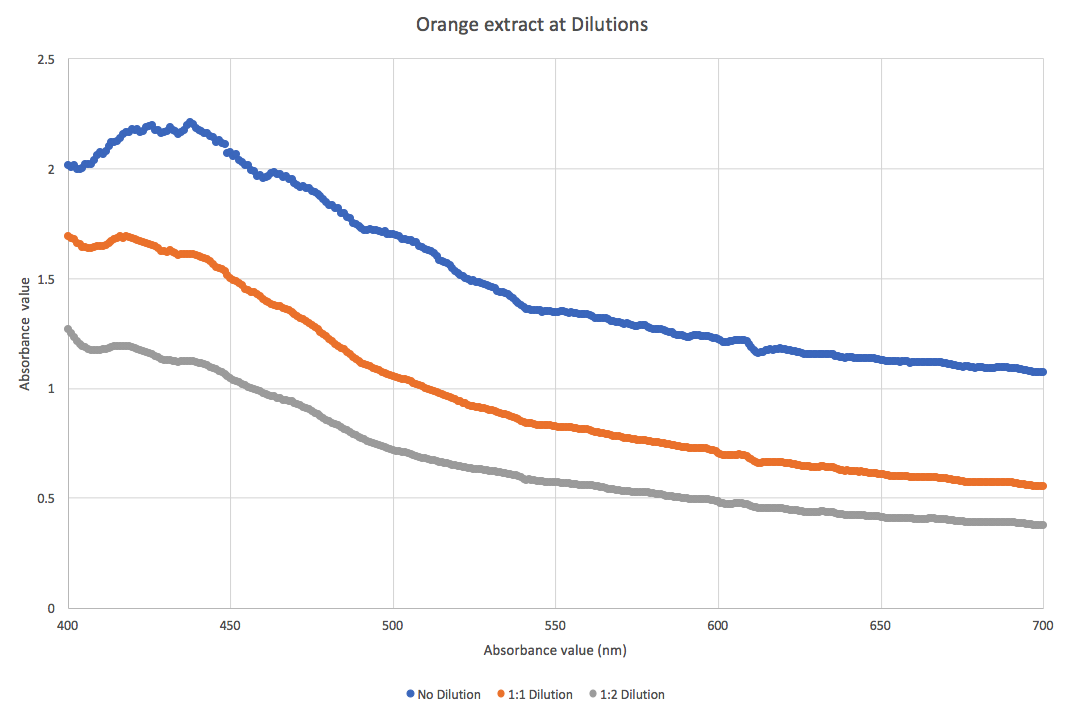
\includegraphics[width=5in]{fig1}\hspace*{\fill}
\caption[Orange extract at various dilutions]{Orange extract at various dilutions}
\end{figure}
\begin{figure}[H]
\hfill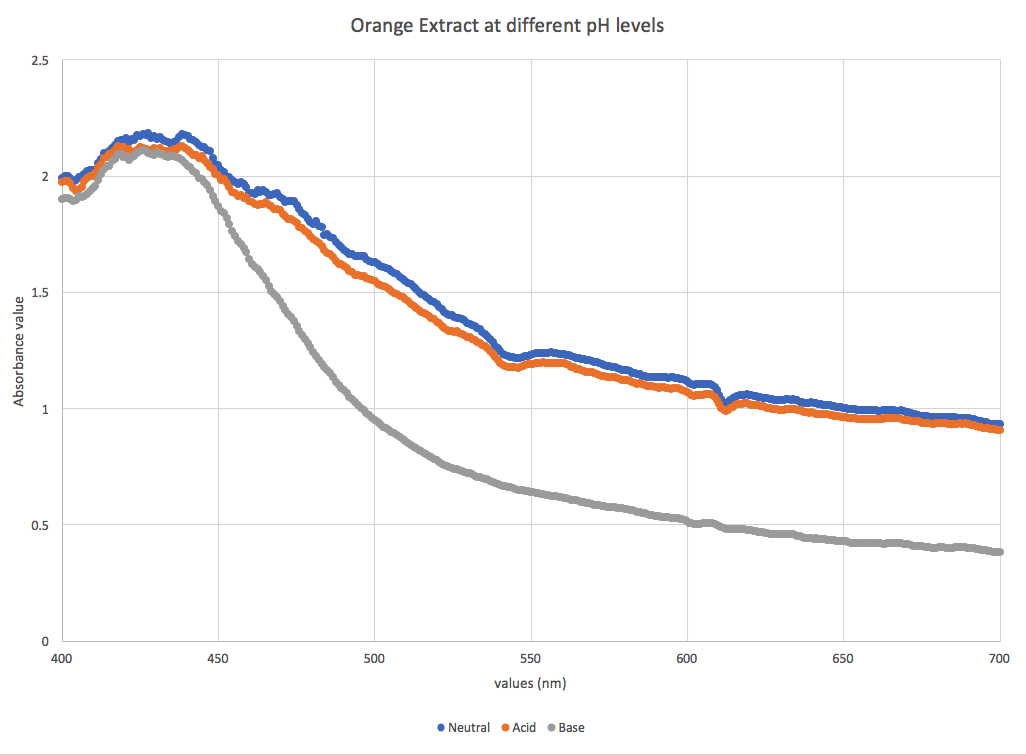
\includegraphics[width=5in]{fig2}\hspace*{\fill}
\caption[Orange extract at different pH values]{Orange extract at different pH values}
\end{figure}
%----------------------------------------------------------------------------------------
%	SECTION 3
%----------------------------------------------------------------------------------------

% \section{Calculations}
% \hspace{5ex}Determining the average volume of unknown container:
% \begin{center}
% Avg. vol. = $\frac{(34.0 ml + 34.0 ml + 31.55 ml + 31.28 ml)}{4}$ = 32.7075 ml \\
% Avg. vol. = 32.71 ml\\
% \end{center}
% \hspace{5ex}Determining volume by mass using density of water:
% \begin{center}
% D = $\frac{m}{v}$ \\
% D = .9977 $\frac{g}{ml}$ \\
% m = 31.21 g \\
% v = ? \\

% .9977 $\frac{g}{ml}$ = $\frac{31.21 g}{v}$ \\
% v =  $\frac{\SI{31.21}{\gram}}{.9977 g}$ ml = 31.28 ml \\
% \end{center}
% \hspace{5ex}Determine the difference error between our groups determined volume and volume determined by the gravimetric method:
% \begin{center}
% Difference error \% = ((experimental value - accepted value)/accepted value)) x 100 \\
% experimental value = 34.0 ml\\
% accepted value = 31.28 ml\\
% difference error = ? \\
% Difference error \% = ((34.0 ml - 31.28 ml)/31.28 ml)) x 100 = 8.695 \\
% Difference error = 8.70 \%
% \end{center}
%----------------------------------------------------------------------------------------
%	SECTION 3
%----------------------------------------------------------------------------------------

\section{Questions}
\hspace{5ex}In this experiment, the solute is the orange and the solvent is the distilled water. The responsibility for the absorbance value lied with the solute. When we applied the solvent to the solute  we get a lower absorbance value. So, we go from a high concentration to a low contraction of solute. The solvent of course absorbs light and we have to zero out the absorbance value before conducting the experiment. The amount of light that is absorbed by the solvent is extensive because it changed the absorbance value. The color of the orange is intensive because even though we diluted the solute, we still get the orange coloring. By changing the acidity, we in-turn changed the color of solution which would bring about a different absorbance value and $\lambda$ max. When we diluted the solution concentration we got a lower absorbance value and $\lambda$ max because the color became a lighter orange. We can assume by either having a stronger concentration or a weaker concentration (diluted). That we will get higher absorbance values (stronger concentration) or lower absorbance values (weak concentration). We can see this by looking at Table 2 and Figure 1 collectively. The relationship that both concentration and absorbance value hold is the concentration is independent because it doesn't need the absorbance value. While the absorbance value, is dependent on the concentration. \\

\hspace{5ex}Visible spectroscopy can't be used to identify a specific compound in this experiment but it could be used to determine the differences concentration.

\end{document}
